\documentclass{beamer}
\usetheme{Madrid}
\usepackage{pgfplots}
\pgfplotsset{compat=1.15}
\usepackage{mathrsfs}
\usetikzlibrary{arrows}
\usepackage[utf8]{inputenc}
\usepackage{xcolor}
\usepackage{hyperref}
\usepackage{fancyvrb}
\usepackage{comment}
\usepackage{listings}
\usepackage{color}
\definecolor{munsell}{rgb}{0.0, 0.5, 0.69}
\definecolor{dkgreen}{rgb}{0,0.6,0}
\definecolor{gray}{rgb}{0.5,0.5,0.5}
\definecolor{mauve}{rgb}{0.58,0,0.82}
\definecolor{minas}{RGB}{0.244, 0.172, 0.36}
\definecolor{PUJ}{RGB}{44, 86, 151}
\definecolor{PUJ2}{RGB}{43, 93, 156}
\definecolor{PUJ3}{RGB}{20, 52, 107}
\definecolor{cyandk}{rgb}{0.0, 0.72, 0.92}
\setbeamerfont{frametitle}{size=\LARGE ,series=\bfseries}
\setbeamercolor{frametitle}{fg=PUJ2, bg=white} %% title of the beamer
\setbeamercolor{titlelike}
{parent=structure,bg=PUJ2}
\setbeamercolor{title}{fg=white, bg=PUJ3} 
%\setbeamercolor{navigation symbols}{fg=white, bg=white}
\setbeamercolor*{palette primary}{use=structure,fg=black,bg=yellow}
\setbeamercolor*{palette secondary}{use=structure,fg=white,bg=PUJ3}
\setbeamercolor*{palette tertiary}{use=structure,fg=white,bg=PUJ3}

\setbeamercolor{block title}{bg=PUJ3,fg=white}


%% code information
\lstset{frame=tb,
  language=Python,
  aboveskip=3mm,
  belowskip=3mm,
  showstringspaces=false,
  columns=flexible,
  basicstyle={\small\ttfamily},
  numbers=none,
  classoffset=1,
  morekeywords={True,False}, keywordstyle=\color{munsell}, 
  classoffset=0, 
  keywordstyle=\color{blue},  
  commentstyle=\color{dkgreen},
  stringstyle=\color{PUJ3},
  numberstyle=\tiny\color{gray},
  breaklines=true,
  breakatwhitespace=true,
  tabsize=4,
}

%% You can change default language in the middle of document with \lstset{language=Java}.


%% PUT or Remove the logo in a slide.


%% Information topic

\institute{Javeriana}
\date{2020}

\title[Pontificia Universidad Javeriana] %optional
{ Introduction a first course in Programming to Data Analysis}
\subtitle{Using python.}

\author[Iván Andrés Trujillo Abella] 
{Iván Andrés Trujilllo Abella}

\institute[] 
{
  Facultad de Ingenieria\\
  Pontificia Universidad Javeriana
  \and
  
\textbf{ trujilloiv@javeriana.edu.co}
}

\date[MITA] % (optional)

\newif\ifplacelogo % create a new conditional
\placelogotrue % set it to true
%\logo{\ifplacelogo\color{red}\rule{.5cm}{.5cm}\fi}
\logo{\ifplacelogo 
\includegraphics[height= 2.0cm]{pujshield.eps}\fi}



\begin{document}



\frame{\titlepage}



\begin{frame}{Contingency table}
\begin{table}[]
\begin{tabular}{lllccc}          &                               &                                & \multicolumn{3}{c}{\textbf{Diagnose}}                                               \\ \cline{4-6} 
          &                               &                                & \multicolumn{1}{l}{Disease} & \multicolumn{1}{l}{} & \multicolumn{1}{l}{No-Disease} \\ \cline{4-6} 
          & \multicolumn{1}{l|}{}         & \multicolumn{1}{l|}{Smoke}     & a                           &                      & b                              \\
\multicolumn{2}{l|}{\textbf{Risk Factor}} & \multicolumn{1}{l|}{}          &                             &                      &                                \\
          & \multicolumn{1}{l|}{}         & \multicolumn{1}{l|}{Not Smoke} & c                           &                      & d                              \\
          &                               &                                & \multicolumn{1}{l}{}        & \multicolumn{1}{l}{} & \multicolumn{1}{l}{}          
\end{tabular}
\end{table}
What it is $P(Disase \mid Smoke) = \frac{a}{a+b}$ 
note that marginal distribution.  Note that $P(Disease \cap Smoke) = \frac{a}{(a+b+c+d)}$. Also note that $P(Smoke)= \frac{a+b}{(a+b+c+d)}$. Note the result of divide the last two probabilities.
\end{frame}




\begin{frame}{Conditional Probability}

The probability of event given a "information".\emph{Probability of $A$ occur given $B$ occurs. }

\begin{equation}
P(A \mid B) = \frac{P(A \cap B)}{P(B)}
\end{equation}

Note that $P(A \cap B)$ it is equal to $P(B \cap A)$.

\begin{equation}
P(A \mid B)P(B) = P(B \mid A)P(A)
\end{equation}
\end{frame}


\begin{frame}{Bayes theorem}
Notice that not is same: 
\emph{The probability that occur A given B, that occur B given A.} However we can compute one of the another.
\begin{equation}
P(A \mid B) = \frac{P(A) P(B \mid A)}{P(B)}
\end{equation}
\end{frame}



\begin{frame}{Bowls problems}
Derive the following problem.
\end{frame}




\begin{frame}{Law of total probability}
The sample space defined as $\Omega$ 
if we split omega in $\omega$ $k$ subsets in order that each $subset$ no overlap with others.
$\bigcup_{i=1}^{k} \omega_{i} = \Omega $ y $
\bigcap_{i=1}^{k} \omega_{i} = \emptyset
$
For instance the sample space defined as $ \Omega= \lbrace a ,b,c,d,e,f\rbrace$
$\omega_{1}=\lbrace a,f \rbrace$  $\omega_{2}=\lbrace b,c,d \rbrace  $ $ \omega_{3}=\lbrace e \rbrace $.
\end{frame}


\begin{frame}{Split $\Omega$}
\begin{figure}

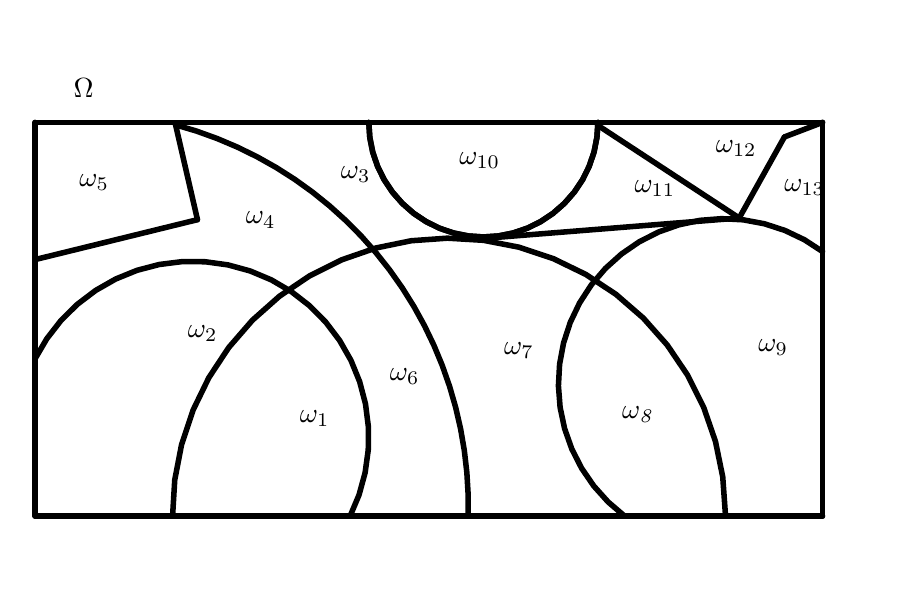
\begin{tikzpicture}[line cap=round,line join=round,>=triangle 45,x=1cm,y=1cm]
\clip(-12.095168341119958,-1.8253174810990838) rectangle (-1.4053738900064559,5.203119715631769);
\draw [line width=2pt] (-12,4)-- (-6,4);
\draw [line width=2pt] (-12,4)-- (-12,-1);
\draw [line width=2pt] (-6,4)-- (-2,4);
\draw [line width=2pt] (-2,4)-- (-2,-1);
\draw [line width=2pt] (-12,-1)-- (-2,-1);
\draw [shift={(-10,0)},line width=2pt]  plot[domain=-0.46364760900080615:2.677945044588987,variable=\t]({1*2.23606797749979*cos(\t r)+0*2.23606797749979*sin(\t r)},{0*2.23606797749979*cos(\t r)+1*2.23606797749979*sin(\t r)});
\draw [shift={(-11.52,-0.88)},line width=2pt]  plot[domain=-0.023899830887098794:1.308676485529425,variable=\t]({1*5.021434058115271*cos(\t r)+0*5.021434058115271*sin(\t r)},{0*5.021434058115271*cos(\t r)+1*5.021434058115271*sin(\t r)});
\draw [shift={(-6.744941662832751,-0.98)},line width=2pt]  plot[domain=0.005697944032979157:3.147290597622772,variable=\t]({1*3.510056979594493*cos(\t r)+0*3.510056979594493*sin(\t r)},{0*3.510056979594493*cos(\t r)+1*3.510056979594493*sin(\t r)});
\draw [shift={(-3.2567368200552362,0.679872248814668)},line width=2pt]  plot[domain=0.9285030181026769:4.07009567169247,variable=\t]({1*2.0979414213033207*cos(\t r)+0*2.0979414213033207*sin(\t r)},{0*2.0979414213033207*cos(\t r)+1*2.0979414213033207*sin(\t r)});
\draw [shift={(-6.30779124440237,4)},line width=2pt]  plot[domain=3.141592653589793:6.283185307179586,variable=\t]({1*1.454939050215934*cos(\t r)+0*1.454939050215934*sin(\t r)},{0*1.454939050215934*cos(\t r)+1*1.454939050215934*sin(\t r)});
\draw [shift={(-6.30779124440237,4)},line width=2pt]  plot[domain=3.141592653589793:6.283185307179586,variable=\t]({1*1.454939050215934*cos(\t r)+0*1.454939050215934*sin(\t r)},{0*1.454939050215934*cos(\t r)+1*1.454939050215934*sin(\t r)});
\draw [line width=2pt] (-12,2.258002259588651)-- (-9.93853929509727,2.764562471815984);
\draw [line width=2pt] (-9.93853929509727,2.764562471815984)-- (-10.218480465012375,3.9776408747814385);
\draw (-11.636643227019698,4.676158017337441) node[anchor=north west] {$\Omega$};
\draw [line width=2pt] (-2,4)-- (-2.4843671441318684,3.8153244435494);
\draw [line width=2pt] (-2.4843671441318684,3.8153244435494)-- (-3.0587180577304687,2.7858275229481317);
\draw [line width=2pt] (-4.851660403825104,3.9608761613021164)-- (-3.0587180577304687,2.7858275229481317);
\draw [line width=2pt] (-6.4346664749495215,2.516316534266319)-- (-3.0587180577304687,2.7858275229481317);
\draw (-8.76230669086882,0.46730808940221685) node[anchor=north west] {$\omega_{1}$};
\draw (-6.736583798724393,3.7454204722981066) node[anchor=north west] {$\omega_{10}$};
\draw (-7.619415734827877,0.9942697876965457) node[anchor=north west] {$\omega_{6}$};
\draw (-6.168560149913624,1.3296090502474822) node[anchor=north west] {$\omega_{7}$};
\draw (-2.9383533759535907,1.3638273423445166) node[anchor=north west] {$\omega_{9}$};
\draw (-4.669798956063524,0.515213698338065) node[anchor=north west] {$\mathit{\omega_{8}}$};
\draw (-11.561362984406223,3.4648304771024248) node[anchor=north west] {$\omega_{5}$};
\draw (-8.2421886509939,3.560641694974121) node[anchor=north west] {$\omega_{3}$};
\draw (-4.512394812417166,3.3895502344889494) node[anchor=north west] {$\omega_{11}$};
\draw (-10.185787642105446,1.548606119668502) node[anchor=north west] {$\omega_{2}$};
\draw (-3.479002391086732,3.8959809575250577) node[anchor=north west] {$\omega_{12}$};
\draw (-2.6098577718220617,3.4032375513277633) node[anchor=north west] {$\omega_{13}$};
\draw (-9.446672532809506,2.985774387743944) node[anchor=north west] {$\omega_{4}$};
\end{tikzpicture}
\end{figure}
\end{frame}

\begin{frame}{$P(A)$}{total law probability}
We need remember by set theory that a event $A$ could be rewrite as $A  = (A \cap B) \cup (A \cap C)$. 
if $(B \cup C ) = \Omega $
for this case we can rewrite 
\begin{equation}
\begin{split}
A &= (A \cap \omega_{1}) \cup ( A \cap \omega_{2})...(A \cap \omega_{k})
\\
P(A)&= P(A \cap \omega_{1}) + ... + P(A \cap \omega_{k})
\\
P(A) &= P( A \mid \omega_{1} )P(\omega_{1}) + P(A \mid \omega_{2}  )P(\omega_{2}) +...+  P( A \mid \omega_{k})P(\omega_{k})
\end{split}
\end{equation}

note that  by total law $P(A)$ 
\end{frame}


\begin{frame}{Monty hall}{Reach the famous in 1990}
There are three closed doors, 
and you must select one to win  a car, behind of the only one, there is a car, and behind the other two there are goats.

and after select the door, another door with a goat it is showed, you must remain in the selected door or switch?

initial probality it is the 1/3.

\end{frame}


\begin{frame}{Monty Hall simulation}
This so not intuitive that generated controversy in the academic community.
\end{frame}



\begin{frame}
The following Figure \ref{fig} show the relation among the probability of two coincidences among two person in the sample.
\begin{figure}[htbp]
\centerline{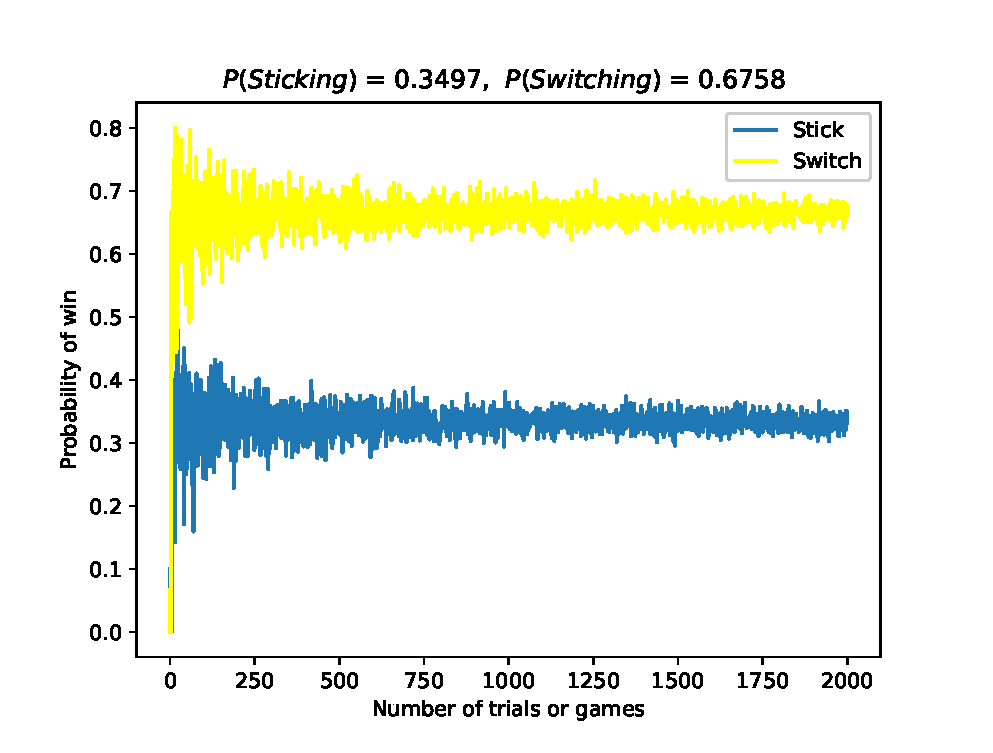
\includegraphics[scale=0.8]{./graphs/Monty.eps}}
\caption{Monty Hall simulation}
\label{fig}
\end{figure}
\end{frame}





\begin{frame}[fragile]{Monty Hall problem}{Python code}
\begin{lstlisting}
def monty_game():
  doors=[1,2,3]
  doors_variable = doors.copy()
  winner = random.randint(1,3)
  select_one = random.randint(1,3)
  values = [winner,select_one]
  switch = list( set(doors) - set(values))
  select_two = random.randint(switch[0], switch[-1])
  s1,s2 = 0,0
  if winner == select_one:
    s1 += 1
  else:
    s2 +=1
  return [s1,s2]
\end{lstlisting}
\end{frame}

\begin{frame}[fragile]{Monty Hall problem}{python code}
\begin{lstlisting}
games=1000
s1_total = []
s2_total = []
for trials in range(1,games):
  values_s1 = sum([monty_game()[0] for _ in range(trials)]) / trials
  s1_total.append(values_s1)
  values_s2 = sum(monty_game()[1] for _ in range(trials)) / trials 
  s2_total.append(values_s2)
plt.plot(np.arange(1,games),s1_total)
plt.plot(np.arange(1,games),s2_total)
print(s1_total[-1], s2_total[-1])
\end{lstlisting}
\end{frame}

\begin{frame}{Monty Hall}{Bayesian solution}
The event $D_{i}$ the $i$ winner door and  $M_{j}$ monty open $j$ door, for $i,j=1,2,3$.

\begin{equation}
P(D_{i} \mid M_{j}) = \frac{P(M_{j} \mid D_{i})P(D_{i})}{P(M_{j})}
\end{equation}

you select the first door  and monty the second, therefore the question  is $P(D_{3} \mid M_{2})$.
Notice that $ P(M_{2}) = \sum_{i=1}^{3} P(M_{2} \mid D_{i}) $.  
given the rules of games, 
$P(M_{2} \mid D_{2}) = 0$, and 
$P(M_{2} \mid D_{3}) = 1$, if monty could select random in two choices $P(M_{2} \mid C_{1})=1/2$ and finally, switch strategy have a probability of 2/3.
\end{frame}






\begin{frame}{Buffon Needled}
\begin{columns}

\column{0.5\textwidth}
Here we have a column


\column{0.5\textwidth}

we have another column


\end{columns}

\end{frame}


\begin{frame}[fragile]{$\pi$ Number}

\begin{columns}


\column{0.5 \textwidth}
\begin{lstlisting}
import numpy as np
import matplotlib.pyplot as plt
dots = 5000
c1,c2=-1,1
x = np.random.uniform(c1,c2, size=dots)
y = np.random.uniform(c1,c2, size=dots)
coordenates_circle = (x**2)+(y**2) < 1
circle_y=y[coordenates_circle]
circle_x=x[coordenates_circle]
pi = 4*sum(coordenates_circle) / dots
plt.scatter(x,y, color='yellow')
plt.scatter(circle_x,circle_y)
\end{lstlisting}

\column{0.5 \textwidth}
What is the probability of a drop lands in the circle?
\begin{equation}
P(hit) = \frac{\pi r^{2}}{4r^{2}}
\end{equation}
\begin{figure}
\centerline{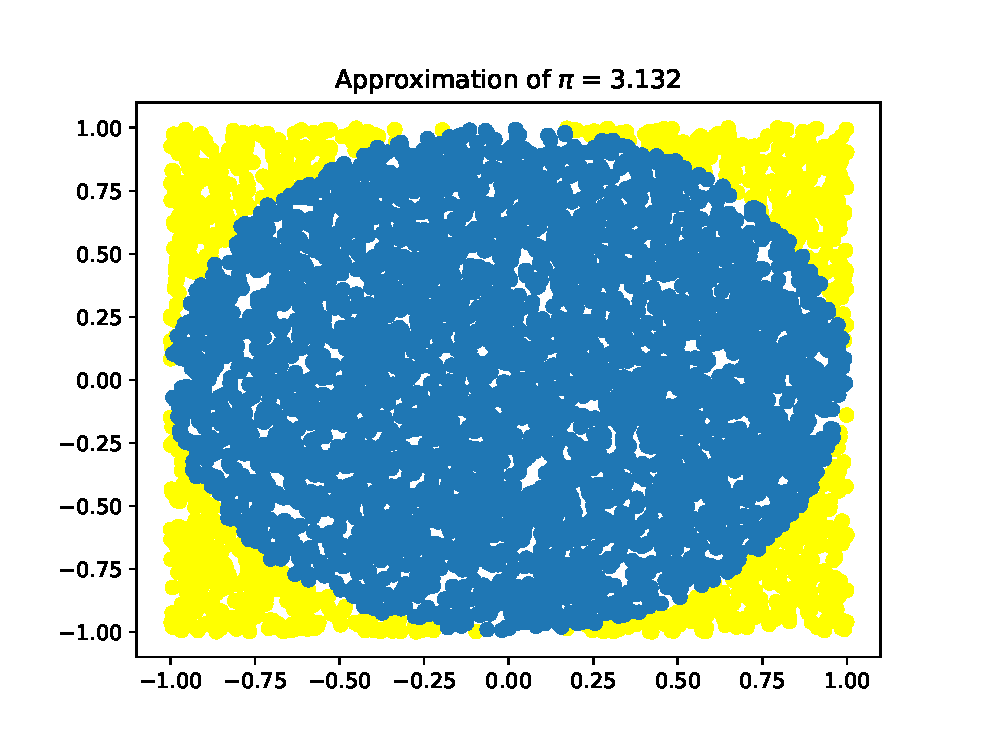
\includegraphics[scale=0.4]{./graphs/PiOne.eps}}
\label{fig}
\end{figure}
\end{columns}
\end{frame}



\begin{frame}{Needles}
Proposed by and resolved by the naturalist. take in mind the 
\begin{figure}
\definecolor{ududff}{rgb}{0.30196078431372547,0.30196078431372547,1}
\begin{tikzpicture}[line cap=round,line join=round,>=triangle 45,x=1cm,y=1cm]
\clip(-12.564766534876606,0.22190923729896378) rectangle (-2.0940558311248365,7.241112822647047);
\draw [line width=2pt] (-12,6)-- (-12,1);
\draw [line width=2pt] (-10,6)-- (-10,1);
\draw [line width=2pt] (-8,6)-- (-8,1);
\draw [line width=2pt] (-4,6)-- (-4,1);
\draw [line width=2pt] (-6,6)-- (-6,1);
\draw [line width=2pt] (-12,6)-- (-4,6);
\draw [line width=2pt] (-12,1)-- (-4,1);
\draw [line width=2pt] (-10,4)-- (-9,4);
\draw [line width=2pt] (-8.296193565998552,2.4731031062869198)-- (-7.5965657346611755,3.0081126243684424);
\draw [line width=2pt] (-10.381358867239362,2.418230335201635)-- (-9.681731035901985,1.938093588205397);
\draw [line width=2pt] (-4.468817782799958,3.3922220219654338)-- (-5.2096001924513,2.8572125038839107);
\draw [line width=2pt] (-6.965528867180401,4.571986600299049)-- (-6.1012827225871735,4.242749973787341);
\draw [line width=2pt] (-7.1164289876649365,1.4579568412091586)-- (-6.238464650300384,1.1424384074687728);
\begin{scriptsize}
\draw [fill=ududff] (-9,4) circle (2.5pt);
\draw [fill=ududff] (-8.296193565998552,2.4731031062869198) circle (2.5pt);
\draw [fill=ududff] (-10.381358867239362,2.418230335201635) circle (2.5pt);
\draw [fill=ududff] (-4.468817782799958,3.3922220219654338) circle (2.5pt);
\draw [fill=ududff] (-6.965528867180401,4.571986600299049) circle (2.5pt);
\draw [fill=ududff] (-6.238464650300384,1.1424384074687728) circle (2.5pt);
\end{scriptsize}
\end{tikzpicture}
\end{figure}
\end{frame}




\begin{frame}[fragile]{Uniform distribution}
\begin{columns}
\column{0.5 \textwidth}
$\mathbf{x} \sim U(a,b)$ in the interval$(a,b)$.
\begin{equation}
f(x) = \frac{1}{b-a}
\end{equation}
the function is defined in the open interval  $a<x<b$.
Remember that:
\begin{equation}
F(x) = \int_{- \infty}^{x}f(u)du
\end{equation}

\column{0.5\textwidth}
\begin{lstlisting}
import numpy as np
np.random.uniform(a,b ,size=(k,p)) # [)

#Draw k list with p elements with numbers [a,b)
\end{lstlisting}
Choose a point in the interval (a,b), you can calculate what it is the probability that a point is in (c,d) 
\end{columns}
\end{frame}

\end{document}